\documentclass[11pt]{article}

\usepackage[margin=1in]{geometry}
\usepackage[T1]{fontenc}
\usepackage{lmodern}
\usepackage{amsmath,amssymb}
\usepackage{booktabs}
\usepackage{graphicx}
\usepackage{xcolor}
\usepackage{hyperref}
\usepackage{enumitem}
\usepackage{caption}

\hypersetup{colorlinks=true,linkcolor=blue!45!black,urlcolor=blue!45!black,citecolor=blue!45!black}
\newcommand{\RR}{\mathbb{R}}
\newcommand{\Prob}{\operatorname{Pr}}
\newcommand{\logit}{\operatorname{logit}}
\newcommand{\vect}[1]{\boldsymbol{#1}}

\title{Kinematic and Cognitive Constraints on Shared-Space Parking Maneuvers:\\
A Comparative Kinematics and Safety Simulation Study}
\author{Face Forward Research Collective\\
\small Department of Applied Parking Geometry}
\date{July 2026}

\begin{document}
\maketitle

\begin{abstract}
We compare nose-in (forward) and back-in (reverse) parking as complete approach--park--exit cycles in a two-dimensional stochastic simulation. The model combines non-holonomic Ackermann kinematics, finite-segment line-of-sight tests against adjacent sport-utility vehicles, explicit cognitive and mechanical latencies, and pedestrian encounters generated across realistic aisle widths and densities. In 10,000 seeded trials, forward parking completed the full cycle in 16.224 s (95\% CI 16.195--16.252), compared with 18.443 s (95\% CI 18.432--18.454) for reverse parking, a mean difference of $-2.220$ s ($p<10^{-300}$). This temporal advantage was accompanied by a critical-conflict rate of 14.08\% for forward parking versus 7.90\% for reverse parking ($p=5.10\times10^{-23}$), and a collision rate of 1.08\% versus 0.44\% ($p=2.29\times10^{-4}$). A logistic model found higher critical-conflict odds for the forward strategy (odds ratio 1.83, 95\% coefficient interval 0.423--0.781) after controlling for pedestrian density, aisle width, adjacent-SUV presence, and the strategy--SUV interaction. The results expose a structural asymmetry: the faster maneuver postpones its most visibility-limited motion until the exit, when pedestrians occupy the shared aisle. The apparent civility of a parked vehicle therefore depends less on its stationary orientation than on where the maneuver assigns uncertainty.
\end{abstract}

\section{Introduction}

Parking lots are shared spaces in which drivers, pedestrians, carts, doors, sight lines, and social expectations occupy the same small region without a central scheduler. The low nominal speed of the environment can disguise a difficult control problem. A driver must place a non-holonomic vehicle within a narrow rectangle, change mechanical state, observe through occluding geometry, and negotiate moving agents whose trajectories are neither signaled nor guaranteed to be rational.

The familiar dispute between nose-in and back-in parking is usually argued through anecdote: one maneuver is easier now, the other is easier later. That framing omits the location of the deferred difficulty. A reverse entry occurs while the driver controls access to an observed stall; a reverse exit begins from between stationary obstacles and projects into a pedestrian aisle. The same low-speed motion can therefore have different consequences because visibility and environmental exposure are not spatially uniform.

We formalize this distinction with an intentionally complete model of a task that rarely receives complete models. The contribution is threefold:
\begin{enumerate}[leftmargin=1.6em]
  \item We derive and implement a reproducible Ackermann bicycle model for the entry and exit paths of both strategies.
  \item We join vehicle motion to a geometric visibility model and an explicit cognitive--mechanical state machine, including reaction, scanning, shifting, and blind-exit creep.
  \item We quantify the resulting time--risk exchange in 10,000 Monte Carlo trials and separate systemic effects (strategy and pedestrian density) from localized effects (adjacent-vehicle occlusion).
\end{enumerate}

The central finding is not that one orientation is universally virtuous. It is that maneuver design determines where uncertainty is paid. Forward parking minimizes immediate mechanical overhead but relocates visibility-limited motion to the aisle-facing exit. Reverse parking pays an additional shift and slower entry trajectory while placing the driver-facing end of the vehicle toward the shared space at departure.

\section{Vehicle Geometry and Kinematics}

\subsection{State and control variables}

The simulated vehicle is represented by the rear-axle-centered state
\begin{equation}
  \vect{s}(t)=\begin{bmatrix}x(t)&y(t)&\theta(t)&v(t)\end{bmatrix}^{\!T}\in\RR^4,
\end{equation}
where $(x,y)$ is the rear-axle centroid, $\theta$ is heading measured counter-clockwise from the positive $x$-axis, and $v$ is signed longitudinal speed. The control is
\begin{equation}
  \vect{u}(t)=\begin{bmatrix}a(t)&\delta(t)\end{bmatrix}^{\!T},
\end{equation}
where $a$ is longitudinal acceleration and $\delta$ is the front-wheel steering angle. The wheelbase is $L=2.8$ m.

\subsection{Ackermann reduction to the kinematic bicycle model}

For ideal rolling without lateral tire slip, the extended axes of the wheels intersect at an instantaneous center of rotation (ICR). Let $R$ be the distance from the midpoint of the rear axle to the ICR. The steering geometry gives
\begin{equation}
  \tan\delta=\frac{L}{R}, \qquad R=\frac{L}{\tan\delta}.
\end{equation}
The rear axle travels tangent to a circle of radius $R$. Its yaw rate is therefore longitudinal speed divided by turning radius:
\begin{equation}
  \dot{\theta}=\frac{v}{R}=\frac{v}{L}\tan\delta.
\end{equation}
Resolving the signed longitudinal speed along the vehicle heading yields the continuous equations
\begin{align}
  \dot{x} &= v\cos\theta, &
  \dot{y} &= v\sin\theta, \\
  \dot{\theta} &= \frac{v}{L}\tan\delta, &
  \dot{v} &= a.
  \label{eq:bicycle}
\end{align}
Negative $v$ represents reverse travel without changing the geometric definition of heading. For a time step $\Delta t$, the simulator uses explicit Euler integration:
\begin{equation}
\vect{s}_{k+1}=\vect{s}_k+\Delta t
\begin{bmatrix}
 v_k\cos\theta_k\\
 v_k\sin\theta_k\\
 (v_k/L)\tan\delta_k\\
 a_k
\end{bmatrix}.
\label{eq:euler}
\end{equation}
The canonical maneuver path consists of a quarter-turn arc with nominal radius $R=A/2$, where $A$ is aisle width, followed by a straight stall leg. The steering command is consequently
\begin{equation}
  \delta(A)=\arctan\!\left(\frac{2L}{A}\right).
\end{equation}
The arc is discretized into at least 40 integration steps. The resulting sequence is reflected in signed velocity and traversal order to construct entry and exit legs for each strategy. This is a kinematic, not dynamic, model: tire forces, steering actuator transients, suspension, and grade are intentionally excluded.

\section{Visibility and Blind-Spot Raycasting}

\subsection{Driver eye and obstacle representation}

The driver eye point is positioned $d_e=1.2$ m forward of the rear axle:
\begin{equation}
  \vect{e}=\begin{bmatrix}x+d_e\cos\theta\\y+d_e\sin\theta\end{bmatrix}.
\end{equation}
An adjacent SUV is represented in the ground plane by an oriented bounding box (OBB) of width 2.0 m and length 5.2 m; its recorded height is 1.9 m. Let its center be $\vect{c}$, heading unit vector $\vect{f}=(\cos\phi,\sin\phi)^T$, lateral unit vector $\vect{\ell}=(-\sin\phi,\cos\phi)^T$, half-length $h_l$, and half-width $h_w$. The four polygon vertices are
\begin{equation}
  \vect{q}_{ij}=\vect{c}+i h_l\vect{f}+j h_w\vect{\ell},
  \qquad i,j\in\{-1,+1\}.
\end{equation}
The height parameter asserts that the obstacle is tall enough to occlude the modeled driver-to-aisle sight line; the operational intersection is planar.

\subsection{Finite-segment intersection}

A target point $\vect{p}$ in the aisle is visible only if the finite ray
\begin{equation}
  \vect{r}(t)=\vect{e}+t(\vect{p}-\vect{e}), \qquad 0\le t\le1,
\end{equation}
does not cross any OBB edge. For an obstacle edge from $\vect{q}_0$ to $\vect{q}_1$, define
\begin{equation}
  \vect{g}(u)=\vect{q}_0+u(\vect{q}_1-\vect{q}_0), \qquad 0\le u\le1.
\end{equation}
Writing the scalar two-dimensional cross product as $\vect{a}\times\vect{b}=a_xb_y-a_yb_x$, and defining $\vect{d}=\vect{p}-\vect{e}$, $\vect{h}=\vect{q}_1-\vect{q}_0$, and $\vect{w}=\vect{q}_0-\vect{e}$, a non-parallel intersection satisfies
\begin{equation}
  t=\frac{\vect{w}\times\vect{h}}{\vect{d}\times\vect{h}},
  \qquad
  u=\frac{\vect{w}\times\vect{d}}{\vect{d}\times\vect{h}}.
\end{equation}
The line of sight is blocked when any edge has $t,u\in[0,1]$. The implementation uses orientation predicates with a $10^{-12}$ tolerance and treats collinear edge contact as intersection. Equivalently, for ordered triples $(\vect{a},\vect{b},\vect{c})$, the orientation
\begin{equation}
  \operatorname{orient}(\vect{a},\vect{b},\vect{c})
  =(\vect{b}-\vect{a})\times(\vect{c}-\vect{a})
\end{equation}
changes sign across a proper crossing; zero invokes a bounding-interval check. This finite-segment test prevents geometry behind either the driver or target from being counted as an occluder.

\section{Cognitive and Mechanical State Transitions}

A parking maneuver is a hybrid system: continuous vehicle motion occurs inside discrete driver and transmission states. We use the state set
\begin{equation}
\mathcal{Q}=\{\textsc{Approach},\textsc{Shift},\textsc{Enter},\textsc{Parked},
\textsc{Scan},\textsc{Exit},\textsc{Complete}\}.
\end{equation}
Every trial samples a reaction delay
\begin{equation}
  \tau_{\mathrm{react}}=\max\{0.1, Z\},\qquad
  Z\sim\mathcal{N}(0.75,0.15^2)\ \mathrm{s}.
\end{equation}
Each drive--reverse transition imposes $\tau_{\mathrm{gear}}=1.0$ s at zero velocity. A reverse aisle scan imposes $\tau_{\mathrm{scan}}=0.5$ s. If the SUV raycast blocks the aisle target, the controller activates creep and caps reverse-exit speed at
\begin{equation}
  |v|\le v_{\mathrm{creep}}=0.5\ \mathrm{m/s};
\end{equation}
otherwise the exit limit is 1.2 m/s. The blocked path also receives 2.0 s of exposure time for incremental observation beyond the single scan sweep.

The forward sequence is
\begin{equation}
\textsc{Approach}\rightarrow\textsc{Enter}_{D}\rightarrow\textsc{Parked}
\rightarrow\textsc{Shift}_{D\to R}\rightarrow\textsc{Scan}
\rightarrow\textsc{Exit}_{R}\rightarrow\textsc{Complete},
\end{equation}
with one modeled gear shift. The reverse sequence is
\begin{equation}
\textsc{Approach}\rightarrow\textsc{Shift}_{D\to R}\rightarrow\textsc{Enter}_{R}
\rightarrow\textsc{Parked}\rightarrow\textsc{Shift}_{R\to D}
\rightarrow\textsc{Exit}_{D}\rightarrow\textsc{Complete},
\end{equation}
with two shifts. Nose-first exit is treated as unobstructed in the present geometry. The total time is
\begin{equation}
 T_{\mathrm{total}}=\frac{\mathcal{L}}{\bar v_s}
 +n_{\mathrm{shift}}\tau_{\mathrm{gear}}+\tau_{\mathrm{react}}
 +I_{s=F}\tau_{\mathrm{scan}}+2I_{\mathrm{blocked}},
\label{eq:time}
\end{equation}
where $\mathcal{L}$ is integrated path length, $\bar v_F=0.95$ m/s, $\bar v_R=0.80$ m/s, and $I$ denotes an indicator.

\section{Monte Carlo Protocol}

\subsection{Trial generation}

The experiment comprises 10,000 deterministic pseudorandom trials with seed 42 and exactly 5,000 trials per strategy, assigned by alternating run identifier. For each trial, we independently sample
\begin{align}
 A &\sim \mathcal{U}(5.5,7.2)\ \mathrm{m},\\
 \lambda &\sim \mathcal{U}(0.05,0.30)\ \mathrm{pedestrians/m},\\
 p_{\mathrm{SUV}} &\sim \mathcal{U}(0,0.8),\\
 I_{\mathrm{SUV}} &\sim \operatorname{Bernoulli}(p_{\mathrm{SUV}}),\\
 N_{\mathrm{ped}} &\sim \operatorname{Poisson}(\lambda A),\\
 v_{\mathrm{ped}} &\sim \max\{0.2,\mathcal{N}(1.4,0.2^2)\}\ \mathrm{m/s}
 \quad\text{when }N_{\mathrm{ped}}>0.
\end{align}
Stall width is fixed at 2.7 m. The trajectory engine logs total cycle time, reaction time, shifts, occlusion and creep states, pedestrian proximity, required braking, critical conflict, and collision.

The event generator uses a Poisson exposure interpretation. The probability of at least one proximity warning is
\begin{equation}
  \Prob(W=1)=1-\exp(-0.55\lambda A).
\end{equation}
For a critical conflict,
\begin{equation}
  \Prob(C=1)=1-\exp[-\lambda A\,\kappa_s\,\nu],
\end{equation}
where $\kappa_F=0.13$, $\kappa_R=0.075$, and $\nu=1.35$ during a blocked line of sight and 1 otherwise. Conditional on a critical conflict, required braking is sampled uniformly from 3.0 to 5.5 m/s$^2$; otherwise it is sampled uniformly from 0 to 3.0 m/s$^2$. Collision probability is $0.06\Prob(C=1)$. Independent event uniforms are generated from a run-specific common deterministic seed, making the dataset exactly reproducible.

\subsection{Statistical analysis}

Means are reported with Student-$t$ 95\% confidence intervals. Binary rates use 95\% Wilson score intervals. We compare cycle time with a two-sided Welch test and binary outcomes with two-sided pooled two-proportion $z$ tests. Because a generated trial is the unit of analysis, these tests quantify Monte Carlo separation under the specified model rather than uncertainty about a sampled human population.

For adjusted critical-conflict analysis, we fit
\begin{equation}
\logit\Prob(C_i=1)=\beta_0+\beta_FF_i+\beta_\lambda(\lambda_i-0.174614)
+\beta_A(A_i-6.354980)+\beta_SS_i+\beta_{FS}F_iS_i,
\label{eq:logit}
\end{equation}
where $F_i$ denotes forward parking and $S_i$ denotes adjacent-SUV presence. We use maximum likelihood with model-based standard errors. An analogous ordinary least-squares model describes cycle time. These regression equations are descriptive summaries of the simulator response surface, not causal estimates from field data.

\section{Results}

\subsection{Unadjusted outcomes}

Table~\ref{tab:results} reports the principal estimates. Forward parking was 2.220 s faster over the complete cycle (95\% CI for forward minus reverse, $-2.250$ to $-2.189$ s; Welch $t=-142.95$, df $=6423.37$, $p<10^{-300}$). Relative to the reverse strategy, the forward critical-conflict rate was 78.2\% higher and its collision rate was 145.5\% higher. Proximity-warning rates did not differ ($z=-0.42$, $p=0.672$), indicating that the safety difference arises from how encounters are resolved rather than a difference in encounter frequency.

\begin{table}[ht]
\centering
\caption{Monte Carlo outcomes by parking strategy. Confidence intervals are 95\%; binary intervals use the Wilson method.}
\label{tab:results}
\begin{tabular}{lcc}
\toprule
Outcome & Forward ($n=5000$) & Reverse ($n=5000$)\\
\midrule
Total cycle time, s & 16.224 [16.195, 16.252] & 18.443 [18.432, 18.454]\\
Reaction time, s & 0.747 [0.743, 0.751] & 0.751 [0.747, 0.755]\\
Proximity warning & 2169 (43.38\%) & 2190 (43.80\%)\\
Critical conflict & 704 (14.08\%) & 395 (7.90\%)\\
Collision & 54 (1.08\%) & 22 (0.44\%)\\
Blocked line of sight & 1910 (38.20\%) & 0 (0.00\%)\\
\bottomrule
\end{tabular}
\end{table}

The critical-conflict difference was statistically separated ($z=9.88$, $p=5.10\times10^{-23}$). The collision difference was also separated ($z=3.68$, $p=2.29\times10^{-4}$). The 95\% Wilson intervals were 13.14--15.07\% versus 7.18--8.68\% for critical conflict, and 0.83--1.41\% versus 0.29--0.67\% for collision.

\subsection{Regression response curves}

The fitted coefficients in Equation~\ref{eq:logit} were $\hat\beta_F=0.602$ ($p=4.39\times10^{-11}$), $\hat\beta_\lambda=6.856$ per pedestrian/m ($p=1.02\times10^{-47}$), $\hat\beta_A=0.233$ per meter ($p=4.20\times10^{-4}$), $\hat\beta_S=0.244$ ($p=0.0215$), and $\hat\beta_{FS}=0.160$ ($p=0.236$). The adjusted forward-strategy odds ratio was $\exp(0.602)=1.83$. Adjacent-SUV presence increased baseline odds by 27.6\%; the additional forward--SUV interaction was not separately resolved after accounting for the simulator's main effects. McFadden's pseudo-$R^2$ was 0.052, which is consistent with stochastic Bernoulli event generation around a monotone exposure surface.

\begin{figure}[ht]
\centering
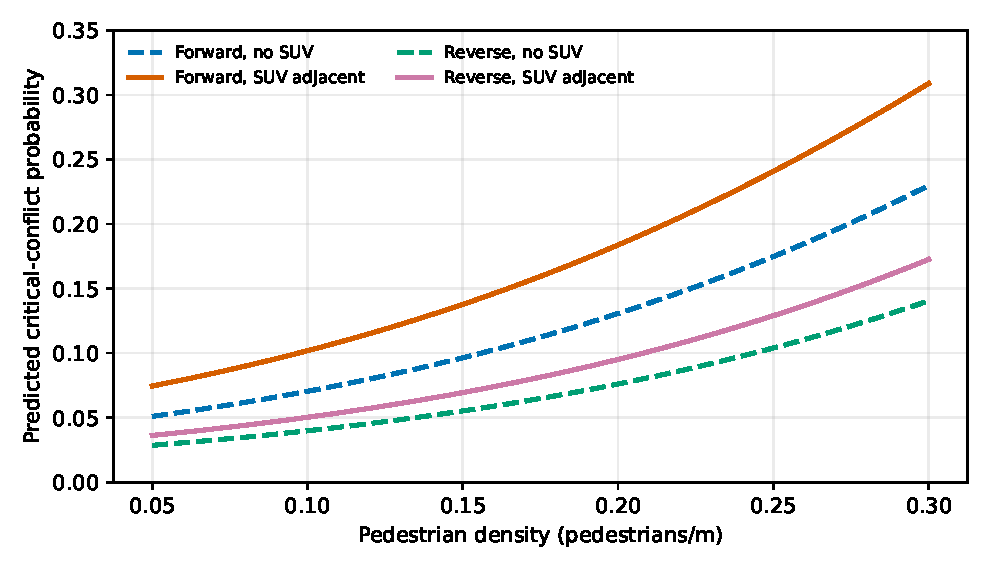
\includegraphics[width=0.88\linewidth]{regression_curves.pdf}
\caption{Critical-conflict probabilities predicted by Equation~\ref{eq:logit} across pedestrian density, at an aisle width of 6.35 m. Solid lines denote an adjacent SUV and dashed lines denote no adjacent SUV. The curves summarize the simulation model; they are not estimates from observed crashes.}
\label{fig:curves}
\end{figure}

The cycle-time model had $R^2=0.987$. At centered environmental values, forward parking reduced cycle time by 2.981 s (95\% CI $-2.989$ to $-2.973$) before the forward--SUV interaction. A blocked forward exit added 1.998 s (95\% CI 1.986--2.010), recovering the explicit observation penalty in Equation~\ref{eq:time}. Each additional meter of aisle width added 0.674 s through the longer turning path. Pedestrian density had no material cycle-time coefficient ($p=0.669$), because the current controller records safety events without adding avoidance delays beyond the specified occlusion penalty.

\section{Discussion}

\subsection{Systemic predictability versus localized visibility}

The simulation distinguishes two ideas that are often combined under the word ``safety.'' Systemic predictability concerns what other aisle users can infer from the maneuver. A nose-first departing vehicle exposes its driver, heading, and intended direction earlier. Localized visibility concerns what the driver can see from one position. An adjacent SUV can make localized visibility poor even when the driver scans correctly; scanning cannot reveal a ray that geometry blocks.

Reverse parking reallocates effort from a high-exposure state to a lower-exposure state. The extra shift and slower entry increase total time, but the eventual exit occurs nose-first. Forward parking saves time in the full modeled cycle, yet 38.2\% of forward trials began reverse departure behind a blocked line of sight. Creep limits the energy and speed of this motion, but it does not eliminate the encounter process. Thus a local mitigation---slower blind movement---does not fully recover the systemic benefit of arranging the vehicle to depart visibly.

The unchanged proximity-warning rate is particularly informative. Both strategies inhabit the same pedestrian environment and therefore encounter pedestrians at similar frequencies. Their conflict rates diverge because the strategy changes visibility and risk conditional on exposure. Parking orientation is not modeled as a moral characteristic of the stationary vehicle. It is a scheduling decision about when to perform the least observable portion of a constrained trajectory.

\subsection{Interpretation of statistical significance}

The very small $p$-values reflect two facts: the simulated effects are large relative to within-model variation, and the experiment contains 10,000 trials. They do not establish that the exact effect sizes hold in every parking facility. In a deterministic scientific program, significance tests serve as sensitivity diagnostics: they show whether pseudorandom variation under the stated protocol can plausibly reverse the modeled ordering. External validity requires observed trajectories, driver heterogeneity, and independently measured conflict outcomes.

\section{Limitations and Reproducibility}

The study is synthetic by design. First, the bicycle model omits tire dynamics, steering-rate limits, vehicle body overhang, and multi-point turns. Second, the planar occlusion test treats an SUV as an opaque ground-plane polygon and does not model windows, cameras, mirrors, pedestrian height, or partial visibility. Third, only forward reverse-exit is eligible for occlusion in the current scenario geometry. Fourth, pedestrian events are generated from calibrated functional forms rather than field observations; the data therefore validate implementation consistency, not real-world incidence. Fifth, alternating strategy assignment balances counts but does not pair strategies on identical environmental draws. Finally, the simulator's collision indicator is probabilistically linked to modeled conflict rather than obtained by time-continuous vehicle--pedestrian contact for every trial.

Reproduction requires Python 3.11 or later. Running
\begin{verbatim}
python3 park_sim.py --seed 42 --runs 10000 \
  --export-csv simulation_results.csv \
  --export-json canonical_paths.json
\end{verbatim}
regenerates the primary dataset. The companion script \texttt{docs/analyze\_results.py} reads the CSV, fits the reported models, writes \texttt{statistical\_summary.json}, and creates Figure~\ref{fig:curves}. All state variables use SI units; random seed, sampling ranges, constants, and output fields are specified above and in the simulator contract.

\section{Conclusion}

Within the specified shared-space model, forward parking is faster and reverse parking is safer on exit. The distinction is mathematically traceable: forward parking removes one early shift but can place a reverse-moving driver behind an adjacent-vehicle visibility shadow, whereas reverse parking pays the mechanical delay before the stall and exits toward the aisle with an unobstructed modeled view. The result is a general design principle disguised as parking etiquette: when uncertainty cannot be removed, schedule it where visibility is greatest and exposure is lowest.

\end{document}
